\documentclass[12pt,a4paper]{scrartcl}
\usepackage[utf8]{inputenc}
\usepackage[ngerman]{babel}
\usepackage[colorlinks=true,
linkcolor=black,
anchorcolor=black,
citecolor=black,
filecolor=black,
menucolor=black,
runcolor=black,
urlcolor=black]{hyperref}
\usepackage{graphicx}
\usepackage{listings}
\usepackage[dvipsnames]{xcolor}
\usepackage[de-DE]{datetime2}
\usepackage{url} \def\UrlBreaks{\do\/\do-}
\usepackage{multicol}
\usepackage{tikz}
\usepackage{float}
\usepackage{pdfpages}

\renewcommand{\baselinestretch}{1.3}

\newcommand{\code}[1]{\texttt{#1}}
\newcommand{\italic}[1]{\textit{#1}}
\newcommand{\boldt}[1]{\textbf{#1}}

\newcommand{\buildAuthors}[1]{
  \begin{multicols}{3}
    \foreach \name\email in {#1} {
      \parbox{\textwidth}{\name \\ \code{\email}}
    }
  \end{multicols}
}

\definecolor{codegreen}{rgb}{0,0.6,0}
\definecolor{codegray}{rgb}{0.5,0.5,0.5}
\definecolor{codepurple}{rgb}{0.58,0,0.82}
%\definecolor{backcolour}{rgb}{0.95,0.95,0.92}

\lstdefinestyle{codestyle}{
    backgroundcolor=\color{white},
    commentstyle=\color{codegreen},
    keywordstyle=\color{magenta},
    numberstyle=\tiny\color{codegray},
    stringstyle=\color{codepurple},
    basicstyle=\ttfamily\footnotesize,
    breakatwhitespace=false,
    breaklines=true,
    captionpos=b,
    keepspaces=true,
    numbersep=6pt,
    showspaces=false,
    showstringspaces=false,
    showtabs=false,
    tabsize=2
}

\lstset{
	numbers=left,
	numberstyle=\small,
	language=bash,
	framexleftmargin=15pt,
	basicstyle=\footnotesize\ttfamily,
	style=codestyle
}


%\lstset{caption={Informationsgewinn}, label=gain-impl}
%\lstinputlisting[firstline=6]{octave/gain.m}

%\begin{figure}
%	\centering
%	\includegraphics[scale=0.6]{img/example1.jpeg}
%	\caption{Beispiel eines Entscheidungsbaumes \cite{example1}}
%	\label{fig:example1}
%\end{figure}

\date{\today}
\title{Teamprojekt - MyUniHelps}

\begin{document}
%\maketitle

\makeatletter
\begin{titlepage}
  \noindent
  \mbox{}\vspace{0.2\textheight}
  \parbox{\textwidth}{\textbf{\Huge \textsf \@title}}
  \raggedright\\
  \vspace{0.2\textheight}
  \large

  % Autoren
  % {Name1}/{Mail1}, {Name2}/{Mail2}, ...
  \buildAuthors{
    {I19}/{myunihelps@hs-harz.de}
  }

  \vspace{0.2\textheight}
  Teamprojekt \\
  Dozent: Sebastian Karius \\
  \normalsize
  \mbox{}\vfill
  Hochschule Harz \\
  Fachbereich Automatisierung und Informatik
\end{titlepage}
\makeatother

%Projektvorstellung 
%	
%	Vorgehensweise
%	
%		Projektverlauf/Teamorganisation (Teams, Aufgaben, Meetings, Zeitplanung)
% 	Vorgehensmodell
%		Code-Reviews
%		Verwendete Tools (dropin, clickup, reports, protokolle)
%		Lösung entstandener Probleme
%	
%	Planung der Softwareentwicklung
%	
%		Prozessmodellierung
%		GUI-Design
%		Entwicklung der Projektwebsite Inhalte
%	
%	
%	Softwarerealisierung
%	
%		E-ID Applikation
%		Projektwebsite
%		Qualitätssicherung
%	
%	Fazit/Schlussbetrachtung
%	Anhang

\pagebreak
\tableofcontents
\pagebreak

\nocite{*}

\section{Projektvorstellung}
Das Ziel dieses Projektes war die Softwareplanung und Umsetzung einer Webapplikation, mit welcher der Austausch von Antragsunterlagen durch ein durch eID gesichertes
System möglich ist.
Das Projekt wurde unter der Leitung von Prof. Dr. Hermann Strack und Sebastian Karius realisiert.
Die Applikation wurde in das Kolibri System des netLabs der Hochschule Harz integriert und sollte für HiWi-Anträge genutzt werden.
Ein Student sollte so in der Lage sein, Dokumente hochzuladen und zu signieren und dies hatte als Ziel die Beschleunigung des Schriftverkehrs, die Nutzbarkeit in Pandemie Situationen und die rechtliche Grundlage für online signierte Dokumente.
Zusätzlich zu dieser Applikation war eine Projektwebsite das Ziel, welche zur Projektvorstellung als auch Anleitung und Unterstützung dient.
Das Projekt lief über das Wintersemester 2021/22 und das Sommersemester 2022.

\section{Vorgehensweise}

\subsection{Projektverlauf/Teamorganisation}
Unser 12 Personen Team wurde während der Entwicklung der einzelnen Softwareelemente in Teilteams aufgeteilt, welche dann die Entwicklung der Features jeweils übernommen haben.
Diese Features wurden in Meetings mit dem Kunden beziehungsweise dem Betreuer aufgestellt und dann im Team intern spezifiziert.
In den Team internen Meetings, welche einmal die Woche stattfanden, wurden Ergebnisse der letzten Woche besprochen und neue Aufgaben an einzelne Mitglieder oder Teams verteilt.
Ergebnisse der Meetings wurde dann in ersten Teil des Projektes in einem Report-Dokument festgehalten, Abschnitt \ref{reports} beschreibt diese ausführlicher.
Zusätzlich zu diesen Reports, welche für den Betreuer vorgesehen waren, wurden Protokolle geführt durch unseren Protokollanten.
Diese Protokolle waren lediglich für das Team gedacht und sollten es ermöglichen jedem Mitglied noch einmal nachzulesen was in einem Meeting geschah.
Dadurch war es auch möglich bei Abwesenheit durch außerordentliche Gründe auf dem Laufenden zu sein, da diese Treffen verbindliche Anwesenheit hatten.
Neben solchen internen Treffen wurden auch einmal die Woche ein Treffen mit den entsprechenden Betreuern gehalten, dort wurden Ergebnisse präsentiert und Feedback zu diesen eingeholt.
Neue Aufgaben wurden geplant oder Anpassungen wurden aufgenommen und zum nächsten Termin vereinbart.
All diese Meetings wurden entweder in Person oder online via Zoom oder Discord abgehalten.
Mithilfe letzteren geschah die gesamte Kommunikation des Teams, zur Organisation der einzelnen Features und deren Zuständen verwendeten wir eine Projektorganisationssoftware namens ClickUp, näheres hierzu wird in \ref{clickup} beschrieben.

Die Zeitplanung fand im ersten Teil des Projektes immer im Wochentakt statt, Aufgaben hatten meistens eine Woche Bearbeitungszeit von der Stellung der Aufgabe im wöchentlichen Meeting mit dem Kunden.
Im zweiten Teil des Projektes, als es um die eigentliche Entwicklung der Webapplikation und ihrer Features sowie der Projektwebsite ging, verschob sich die Zeitplanung.
Aufgrund der Arbeitslast der Entwicklung und anderen Projekten aus anderen Modulen, welche zur gleichen Zeit liefen, konnten die einzelnen Entwicklungsteams ihre eigenen Fristen und Arbeitszeiträume setzten, unter dem Rahmen einer allgemeinen Deadline.
Diese diente dazu zu verhindern, dass Aufgaben zu Lange geplant wurden und somit erst zum Schluss des Projektes angefangen oder beendet wurden.

%Teamrollen
%Gantt Chart
%Zeitplanung

\subsection{Vorgehensmodell}
Als Vorgehensmodell wurde \italic{Feature Driven Development} gewählt.
FDD ist eine agile, iterative Methode, bei welcher eine wertvolle Weiterentwicklung der Software / des Projektes im Vordergrund steht. \cite{fdd}
Aufgrund unserer kurzen Entwicklungszyklen (Sprints) von ca. 2 Wochen, der wöchentlichen Berichterstattungen und unserer Teamorganisation/Erfahrung, wurde FDD anderen Methoden wie Scrum oder den diversen Wasserfallmodellen vorgezogen.

Feature Driven Development sieht vor, ein allgemeines, übergeordnetes Modell zu entwickeln.
Dafür analysieren der Entwicklungsleiter, die Anforderungsmanager, die Architekten und etwaige Domainspezialisten die Problemstellung und aufgestellte Anforderungen \footnote{Domainspezialisten beschränkten sich bei uns auf Teammitglieder mit HiWi-Hintergrund}.
Das für unser Projekt entstandene Modell ist in Abs. \ref{processmodel} beschrieben und abgebildet.

Im nächsten Schritt wird das Modell in Features aufgeteilt, welche von kleinen Teams bearbeitet werden können.
Die Erstellung dieser Featureliste war bei uns die Verantwortung des Entwicklungsleiters, wird aber allgemein auch mit den Architekten und Domainspezialisten erstellt.
Unsere Featureliste ist in Abs. \ref{featureliste} abgebildet.
Die Zeitrahmen wurden in unserem Organisationswerkzeug verwaltet.

Die Planung der Features erfolgt zusammen mit dem Projektleiter und dem Entwicklungsleiter im nächsten Schritt.
Hier werden die Prioritäten und Abhängigkeiten der Features bestimmt und die Bearbeitung dieser in den Zeitplan integriert.
Darüber hinaus wurden unsere Entwickler in diesem Schritt in kleine Entwicklungsteams aufgeteilt, welche jeweils immer Verantwortung für ein Feature übernehmen und dieses bearbeiten.

In der nächsten Phase entwickelt jedes Team ein Design für das jeweilige Feature und implementiert dieses.
Nach dieser Phase befindet sich das Feature in der Review, wobei der Entwicklungsleiter die Codequalität begutachtet und Softwaretester die Funktionalitäten auf die Probe stellen.
Ist dies erfolgt, wo wird das Feature in den Main-Build eingeführt und das Team kann sich auf die nächste Iteration vorbereiten.
Falls Probleme nicht bis Ende der Iteration behoben werden konnten, so wird das Feature in der nächsten Iteration mit eingeplant.

Der Master-Build ist in unserem Team der \code{master}-Branch, konform zur Branching-Strategie unserer Versionskontrolle.
Für diese verwenden wir \italic{Github Flow} \cite{github-flow}.
Diese Strategie gibt 6 Regeln vor, welche von allen Entwicklern im Team eingehalten werden müssen.
Die erste Regel besagt, dass alles im \code{master}-Branch bereit ist zum Bereitstellen.
D.h. nur fertige Features, welche die Review-Phase durchlaufen haben, werden in den \code{master}-Branch gemerged.
Des Weiteren wird jede neue Entwicklung, bei uns sind dies konkret Features, in einem neuen Branch vollzogen und vom Entwicklungsleiter nach der Review in der \code{master} gemerged.
Als Konvention werden diese in unserem Team \code{feature/<feature-name>} genannt, wobei \code{feature-name} der Name aus der Featureliste ist.
In Github-Flow werden Pull-Requests vorgesehen, wenn ein Feature bereit zur Review ist.
Weil wir diese in unserem Projekt nicht zur Verfügung hatten, wurden dafür die Features in unserem Organisationswerkzeug speziell gekennzeichnet.

\subsection{Marketing}

\paragraph{Teamname}
Logischerweise musste ein Teamname her.
Dies gestaltete sich zunächst als schwierig.
Der Teamname sollte kurz, prägnant und einprägsam sein.
Zusätzlich sollte der Name nicht bereits existieren.
Nach längeren Überlegen, Probieren und Abstimmen fiel die Wahl auf "myUniHelps".

\paragraph{Slogan}
Wichtig war es, inhaltlicht mit dem Slogan die Zielgruppen anzusprechen. 
Besagte Zielgruppen sind Hochschulen / Universitäten, Studenten, Dozenten und Personalabteilungen.
Außerdem sollte er einprägsam sein und gut ins Ohr gehen.
Nach längeren Überlegen, Probieren und Abstimmen fiel die Wahl auf "Hiwi-Anträge leicht gemacht! Einfach hochladen.".

\paragraph{Marketingkonzept}
Anfangs musste recherchiert werden, was unter einem Marketingkonzept zu verstehen ist und was inhaltlich dazugehört.
Der erste Punkt im Markteingkonzept war die SWOT-Analyse (SWOT $\rightarrow$ Strength, Weakness, Oppurtunities, Threats).
Dabei wurden die Stärken, Schwächen, Chancen und Risiken analysiert und gegenüber gestellt. Durch Betrachtung dieser 4 Aspekte gingen dann die Marketingziele heraus.
Mithilfe der Marketingstrategien und Marketinginstrumenten sollen diese Ziele dann verwirklicht werden.

\paragraph{Marketingziele}
Hier ist eine Auflistung der bereits erwähnten Marketingziele:
\begin{itemize}
    \item Produktnachfrage erhöhen
    \item Präsenz in den wesentlichen Online Kanälen des Kunden
    \item Erhöhung der Servicequalität
    \item Erhöhung der Kundenzufriedenheit
    \item Prozessoptimierung
    \item Umstieg der allgemeinen Unterschrift zur Qualifizierten Elektronischen Signatur (QES)
\end{itemize}



\begin{figure}[H]
	\centering
	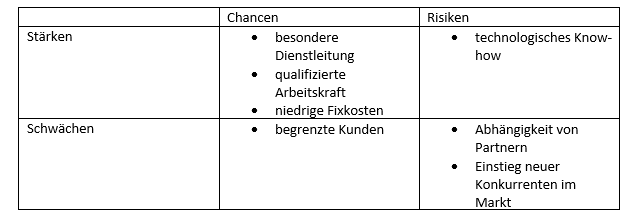
\includegraphics[scale=0.9]{img/SWOT-table.png}
	\caption{SWOT-Analyse}
	\label{fig:use-case}
\end{figure}


\subsection{Code-Reviews}
Neben den Softwaretests und der Qualitätssicherung, wurde während der Entwicklung auch auf die Güte des geschriebenen Quellcodes geachtet.
Diese wurden in der Review-Phase jedes Features vom Entwicklungsleiter vollzogen.
Darüber hinaus haben wir Code-Reviews als weitere Instanz für das Identifizieren von Fehlern im Quellcode herangezogen.
Im Wesentlichen wurden u.a. folgende Kriterien beachtet:

\paragraph{Formatierung}
Darunter fallen u.a. das Einhalten von CamelCase und PascalCase, Dokumentation der Funktionalitäten und das Erstellen von Annotationen im Quellcode.
Insbesondere Letzteres hat bei uns als \glqq Self-Review\grqq  agiert, um eventuelle Fehlerquellen bereits während der Entwicklungsphase der einzelnen Features zu identifizieren und zu beheben.
Darüber hinaus wird hier auch auf einheitliche Formatierung mit dem restlichen Quellcode geachtet.

\paragraph{Architektur}
Darunter versteht sich das Einhalten der festgelegten Softwarearchitektur.
Diese wird bei uns in Abs. \ref{impl} erläutert.

\paragraph{SOLID-Prinzipien}
Von diesen wurde im Wesentlichen nur auf das \italic{Single Responsibility Principle} und das \italic{Dependency Inversion Principle} geachtet.
Während die Einhaltung der anderen Prinzipien ebenfalls Gegenstand der Code-Review war, so haben diese in unserem Design der Software kein große Anwendung gefunden.
Das Single Responsibility Principle besagt, dass eine Klasse nur eine Verantwortung haben sollte.
Dies erhöht die Wiederverwendbarkeit, Wartbarkeit und Lesbarkeit des Quellcodes.
Das Dependency Inversion Principle besagt, dass Klassen auf Abstraktionen und nicht konkreten Implementierungen abhängig sein sollten \cite{Goll.2014}.

\subsection{Verwendete Tools}
\subsubsection{ClickUp}
\label{clickup}
ClickUp ist eine Projektorganisationssoftware, welche wir gewählt haben um Aufgaben, Beschreibung für diese und Unteraufgaben für alle einsehbar zu sammeln.
In diesem Sinne erlaubt ClickUp Aufgaben aufzulisten, diesen Unteraufgaben oder Checklisten hinzuzufügen sowie Personal für diese einzuteilen und Deadlines zu setzten.
Wir haben uns für ClickUp entschieden, da im kostenfreien Kontingent alle Features vorhanden waren die wir benötigten.
Wichtig hierbei war der Umfang dieser Features, anders als andere Softwareangebote unterstützt ClickUp ohne Kosten eine große Menge an Personen, was für unser 12 Personen Team wichtig war.
Ein weiterer Punkt, welcher für uns unverzichtbar war das Vorhandensein eines Kanban Boards um Aufgaben übersichtlich darzustellen und in Kategorien einzuteilen. 
Hierfür wurden Aufgaben in \italic{TODO, IN PROGRESS, REVIEW} und \italic{COMPLETE} eingeteilt.
\italic{REVIEW} markierte Dinge umfassten in unserem Projekt die Qualitätssicherung und die Softwaretestung, erst wenn diese beide Schritte abgeschlossen wurden konnte ein Feature als \italic{COMPLETE} markiert werden.
Näheres zu den jeweiligen Tests wird im Abschnitt \ref{qualitiyassurance} erläutert.
Zusätzlich zu diesen beiden Punkten unterstützt ClickUp Gantt-Charts zur Zeitplanung, welches für uns ein weiter Pluspunkt war.
Diese drei Punkte haben keine andere Softwarelösungen kostenfrei angeboten und wir haben uns daher für ClickUp entschieden.

Tasks konnten ebenfalls Beschreibungen hinzugefügt werden, welche wir für User Stories verwendet haben, um die Features weiter zu definieren.
Ein weiters nützliches Feature sind Tags und Labels, welche Aufgaben hinzugefügt wurden um spezielle Dinge einfach zu visualisieren, wie zum Beispiel die verantwortlichen Teamabteilungen oder eine nötige Datenbankänderung.

DropIn


\subsubsection{Meetingreports und Protokolle}
\label{reports}
%Report Dokument und Protokoll Dokument
\subsection{Lösung entstandener Probleme}

\section{Planung der Softwareentwicklung}

\subsection{Anforderungen}
%features
\label{requirements}

Zu Beginn dieses Projekts stand die allgemeine Anforderungsanalyse auf Basis der Informationen über das derzeitige (nicht digitale) Verfahrenssystems, den rechtlichen Rahmenbedingungen und der 
 Abgrenzung der Aufgabe zu anderen Anwendungen. Die Analyse ergab schnell eine Aufteilung in 3 untereinander abhängige Bereiche. Die klare Definition von Funktionalitäten und Rollen in Form des nachstehenden UseCase-Diagramms, sowie Textform bildete dabei die Grundlage und die erste Begriffsklärung.

\begin{figure}[H]
	\centering
	\includegraphics[scale=0.7]{img/use-case.png}
	\caption{Prozess der HiWi-Anträge}
	\label{fig:use-case}
\end{figure}

Der zweite Bereich umfasst die Analyse der Prozessabläufe, wie sie im nachfolgenden Kapitel vorgestellt werden. Das Aufstellen und Entwickeln von Sicherheitsanforderungen und der Ableitung von Sicherheitsrichtlinien, bzw. eines Sicherheitskonzept ist Teil des dritten Bereichs der Anforderungsanalyse. Bei der Informationsgewinnung wurden verschiedene Quellen neben dem Kunden genutzt, unter anderem die eigenen Erfahrungen mit dem System, sowie allgemeine Regelwerke zum Umgang mit personenbezogenen Daten.

Im weiteren Verlauf des Projekts, zur Umsetzung der Featureliste, wechselte die Arbeitsweise des Teams. Infolgedessen wurde die Anforderungsanalyse neu strukturiert, indem basierend auf eine Featureliste jedes Feature eine eigene Anforderungsanalyse durch den zuständigen Entwickler erfuhr und diese dann durch den Teamleiter, den Anforderungsmanager oder innerhalb eines Team-/Kundenmeetings überprüft wurde. Diese dynamische Herangehensweise erlaubt die Optimierung von Ressourcen und Verteilung der Aufgaben, sowie die Einflussnahme und Ideenfindung neuer Features seitens der Entwickler. 

\subsection{Prozessmodellierung}
\label{processmodel}
Im Folgenden ist der Prozess der Einstellung von HiWi-Anträgen als BPMN-Diagramm abgebildet (Abb. \ref{fig:bpmn-process}).
Die einzelnen Aufgaben / Aktivitäten wurden hier aus den Anforderungen aus Abs. \ref{requirements} abgeleitet und von unseren Stakeholdern \footnote{Von Herrn Strack} bestätigt.
Diese Interaktion ist der Grund, weshalb wir die BPMN als Modellierungssprache über UML o.a. genommen haben.
Die Verarbeitung von Stundenzetteln ist hier nicht mit enthalten.

\begin{figure}[H]
	\centering
	\includegraphics[scale=0.6]{img/eHiWi-process.png}
	\caption{Prozess der HiWi-Anträge}
	\label{fig:bpmn-process}
\end{figure}

\subsection{GUI-Design}

\subsection{Entwicklung der Projektwebseiteninhalte}

\subsection{Planung eines Features}

Das Feature Stundenabrechnung bietet mit seiner aufwendigen Funktionalität und Umfang ein gute Ausgangslage für die Konzeptionierung von Software. Es steht hierbei beispielhaft für die Vorgehensweise der Entwicklung, gleich wolle diese besonders dokumentiert und ausführlich erfolgt war.

\paragraph*{Anforderungsanalyse + Optionsanalyse}

Beginnend mit der Anforderungsanalyse war bekannt, das dieses Feature ungewöhnlich viel Aufwand und Spielräume in der Umsetzung aufweist. Die relativ offene Zielsetzung begünstigte diesen Umstand, wodurch es notwendig wurde vor der Konzeption eine Optionsanalyse, im konkreten Fall der Eingabe- und Verarbeitungsmechanismen durchzuführen. Grundlage hierfür bot das derzeit verwendete Excel-Dokument zur Stundenabrechnung, sowie einige Erfahrungen über Prüf- und Speicherverfahren der Verwaltung als Stakehholder.

\paragraph*{GUI-Oberfläche}

Nach Abschluss der Optionsanalyse und der Entscheidung für ein reines HTML-Formular begann die Konzeptionierung der verschiedenen Bereiche beginnend bei der Planung / testweisen Umsetzung der GUI-Oberfläche als “Einstiegspunkt“ zum Feature und ersten Testversuch für den Beweis der Optionsanalyse. 

\begin{figure}[H]
	\centering
	\includegraphics[scale=0.35]{img/GUI_Demo_Stundenabrechnung.png}
	\caption{Ansicht Demonstrator HTML-Formular des Features Stundenabrechnung}
	\label{fig:bpmn-process}
\end{figure}

\paragraph*{Datenbankschema}

Aufbauend auf der GUI-Oberfläche und der damit ableitbaren Anforderungen auf notwendige Werte und deren Zusammenhang begann die Planung des Datenbankschemas und die entsprechende Übersetzung auf SQL. Während der Analyse wurde zudem festgestellt, dass Teile der Werte berechenbar, bzw. redundant sind. 

Dieser Umstand wurde im finalen Datenbankschema durch den Wegfall der zentralen Monatsansicht, in Abwägung des damit verbundenen Aufwand bei der Generierung des PDFs, berücksichtigt.\\

\begin{figure}[H]
	\centering
	\includegraphics[scale=0.6]{img/ER_Diagramm_Stundenabrechnung.png}
	\caption{Datenbankschema Feature Stundenabrechnung}
	\label{fig:bpmn-process}
\end{figure}

\paragraph*{Prozessmodellierung}

Den dritten Teil der Konzeption umfasste die Prozessmodellierung. Hierbei wird angenommen, dass der Nutzer zuvor verschiedene Einträge (ohne tiefgründige Prüfung) in dem System vorgenommen hat. Der beistehende Programmablaufplan sieht die Verarbeitung der Anfrage einer PDF-Ansicht in Abhängigkeit von ausgewählten Monat und Nutzer vor, wobei das Ergebnis entweder ein fertig ausgefüllter Arbeitsnachweis mit Prüfung oder eine entsprechende Fehlermeldung bei “falschen Daten“.

\begin{figure}[H]
	\centering
	\includegraphics[scale=0.6]{img/AB_Diagramm_Stundenabrechnung.drawio.png}
	\caption{Programmablaufplan PDF-Generierung Feature Stundenabrechnung}
	\label{fig:bpmn-process}
\end{figure}

\paragraph*{Umsetzung}

Nach Abschluss der Konzeption hätte die Umsetzung des Feature unter Abstrichen in der Funktionalität erfolgen sollen. Diese Umsetzung schaffte aber den Schritt über die GUI-Oberfläche nicht hinaus. Dies lag zum einen an Problemen bei der Anpassung der Frontend-Datenbank, welche eigentlich gar nicht dafür gedacht war, der generellen Erreichbarkeit des Gesamtsystems und den damit einhergehenden Ressourcen- und Zeitmangel, aufgrund der späten Anforderung des Features durch den Kunden.

\section{Softwarerealisierung}
\label{impl}
Das \italic{MyUniHelps} System wurde nicht von Grund auf konzipiert und realisiert, sondern als Komponente der Netlab Systemumgebung.
Diese ist mithilfe des Laravel-Frameworks und der Sprache PHP in einer MVC-Architektur \cite{Goll.2014} realisiert.
Unsere Realisierung verfolgt dementsprechend dieselbe Architektur und denselben Technologie-Stack.

\paragraph{Model}
Das Model enthält in einer MVC-Architektur die Geschäftslogik der Anwendung.
Im \italic{MyUniHelps} System ist dies das Verwalten (Erstellen, Bearbeiten und Löschen) von Einstellungsprozessen.
Dazu gehören u.a das Verarbeiten eingehender HiWi-Formulare und das Signieren dieser mittels eIDAS.
Darüber hinaus gehört das Einsehen und Validieren der Daten mit zur Geschäftslogik.
Das Design der Modelle wurde aus den Anforderungen (siehe Abb. \ref{fig:use-case} und \ref{fig:bpmn-process}) abgeleitet.
Aufgrund dessen, dass die Logik für das Signieren, eIDAS und weiteren Funktionalitäten bereits im Projekt der Systemumgebung gegeben waren, beschränkt sich der neu hinzugefügte Quellcode für die Modelle zur Mehrheit nur auf Datenbanktransaktionen.
Lediglich das Auslesen von den PDF-Formularen für die Umsetzung einigen Features ist noch mit enthalten.
Die Kommunikation mit der Datenbank wurde durch die Verwendung von Laravel's Eloquent Komponente, ein Objekt-Relationaler Mapper, ebenfalls trivialisiert.

\paragraph{Controller}
Die Controller verarbeiten die Eingaben von Benutzern bzw. allgemein alle Anfragen in einer Webanwendung innerhalb einer MVC-Architektur.
In der \italic{MyUniHelps} Anwendung beinhaltet dies die Aufrufe der Geschäftslogik der Modelle und das Vorbereiten der Resultate für die Views.

\paragraph{View}
Views bilden die Oberfläche mit welchem der Benutzer mit der Anwendung interagiert.
In unserer Anwendung sind dies ausschließlich HTML-Seiten, welche dynamisch generiert werden.
Das Laravel-Framework stellt die \italic{Blade} Syntax innerhalb von Views (Blade-Dateien) bereit, um die vom Controller zur Verfügung gestellten Daten im HTML einzubetten.
Darüber hinaus erlaubt Blade die Ausführung von PHP-Code innerhalb der Views für weitere, auf Oberflächen bezogene, Logik.
Dies fördert weitergehend das \italic{Seperation of Concerns} Prinzip, welches ebenfalls ein Kriterium für die Code-Reviews war.

\paragraph{eID}
\label{eid}
Damit die Anträge vollständig digital verarbeitet werden können, muss die handschriftliche Unterschrift durch elektronische Methoden realisiert werden.
Um die Anforderung an rechtlich gültigen Unterschriften zu erfüllen, muss nach der eIDAS-Verordnung der EU eine qualifizierte elektronische Signatur vorliegen \cite{Dumortier.2016}.
Hierfür wird die eID-Funktionalität des Personalausweises verwendet, mit welchem ein Benutzer sich bei der \italic{MyUniHelps} Anwendung authentisiert.
Die Anwendung wiederum verwendet die \italic{AusweisApp2} als Schnittstelle zwischen dem Personalausweis und \italic{MyUniHelps}.

Neben der Signatur der Anträge, erlaubt die eID das Auslesen der persönlichen Daten wie Name, Anschrift, etc. des Benutzers.
Diese Daten werden ebenfalls auf den Formularen verlangt und müssen vom Benutzer manuell für jeden Antrag eingetragen werden.
Das System kann hier die Daten automatisch ergänzen 
 \footnote{Weil unser System nur Testbenutzer ohne eID-Integration hatte, mussten diese Daten trotzdem in den Anträgen vorhanden sein.
Die Daten, welche aus der eID ausgelesen werden, wurden hier aus den Formularen ausgelesen und im System für weitere Verarbeitungen hinterlegt}
und verringert somit auch die Anzahl von eventuellen Fehlern in den Formularen.

\subsection{Projektwebseite}
Mit der Marketingwebseite wird das Produkt "myUniHelps" beworben und es soll für den Kunden transparenter gemacht werden.
Zur Entstehung der Marketingwebseite war zunächste wieder Recherche notwendig, um dann über eine geeignete Vorgehensweise nachzudenken.
Nach den Recherchen und das besprechen der Vorgehensweise, ging es an das Entwickeln der Marketingwebseite.
Parallel zur Entwicklung wurden die Inhalte für die Marketingwebseite entworfen.
Die Inhalte sind Slogan, ein kleiner Bereich mit Informationen, Vorteile, eID, QES, Nutzerbewertungen und die Teamvorstellung.

\begin{figure}[H]
	\centering
	
\includegraphics[scale=0.9]{img/marketing.PNG}
	\caption{Marketingwebseite}
	\label{fig:use-case}
\end{figure}

\subsection{Qualitätssicherung}
\label{qualitiyassurance}

\subsection{Einrichten der Infrastruktur/Artefakte}

\paragraph{Installation von Apache2}
Damit die Marketingwebseite und das Laravelprojekt erreichbar sind, mussten die Dateien \code{000-default.conf} und \code{default-ssl.conf} wie folgt bearbeitet werden.

\begin{figure}[H]
	\centering
	\includegraphics[scale=1.0]{img/000-default.conf.png}
	\caption{000-default.conf}
	\label{fig:bpmn-process}
\end{figure}

Durch diese Änderung in der Datei \code{000-default.conf} ist die Marketingwebseite auf dem Port 80 und das Laravelprojekt auf dem Port 8080 für unverschlüsselte Verbindungen erreichbar.
Die Änderungen in der Datei \code{default-ssl.conf} für verschlüsselte Verbindungen sehen dabei wie folgt aus.

\begin{figure}[H]
	\centering
	\includegraphics[scale=0.9]{img/default-ssl.conf.png}
	\caption{default-ssl.conf.png}
	\label{fig:bpmn-process}
\end{figure}

Durch diese Änderungen ist die Marketingwebseite unter dem Port 443 und das Laravelprojekt unter dem Port 8443 erreichbar. Die verwendete SSLCertificateFile und SSLCertificateKeyFile sind dabei mit 2048 bit selbst erstellte lokale Schlüssel, die sich auf dem Server befinden. Nach einem abschließenden Neustart des Apache2 waren beide Seiten erreichbar.

\paragraph{Installation von Git und pdftk}
Die Installation von Git und pdftk verlief problemlos über die Befehle \code{apt install git} und \code{apt install pdftk}.
Es wurde keine weitere Konfiguration benötigt.
Das Teamprojekt wurde über Git in das Verzeichnis \code{/var/www} geladen. Der dafür genutzte Befehl war: \\ \code{git clone git@netlab-project.hs-harz.de:teamproject}.\\
Das Klonen des Projekts war allerdings erst möglich, nachdem im git-Projekt der Schlüssel des Servers zur Berechtigung zum Klonen hinterlegt wurde.
Zusätzlich wurde in diesem Schritt die .env-Datei im Ordner des Laravelprojekts bearbeitet und mit Daten der Datenbank gefüllt, bzw. ersetzt.
Damit wurde dem Projekt vorgegeben, wohin und mit welchen Credentials es sich für die Migration der Datenbank verbinden muss. Die Daten waren dabei Folgende:
\lstset{caption={Datenbankconnection für den Composer}, label=test}
\begin{lstlisting}
DB_CONNECTION=mysql
DB_HOST=localhost
DB_PORT=3306
DB_DATABASE=laravel
DB_USERNAME="root"
DB_PASSWORD=""
\end{lstlisting}

\paragraph{Installation von Composer}
Der Composer benötigt auf Grund der Laravel-Version des Projektes mindestens PHP8, jedoch eine ältere Version als 8.1. Da PHP8 selbst Fehler hervorbrachte, wurde PHP8.0.4 installiert.
Zusätzlich zu PHP8.0.4 wurden zusätzliche PHP-Packages benötigt, die dann ebenfalls installiert wurden. Die benötigten Packages sind die Folgenden.

\begin{itemize}
    \item php8.0.4-zip
    \item php8.0.4-mbstring
    \item php8.0.4-curl
    \item php8.0.4-bcmath
    \item php8.0.4-json
    \item php8.0.4-xml
    \item php8.0.4-tokenizer
\end{itemize}

\paragraph{Installation der Datenbank}
Für das Projekt wurde mariadb verwendet. Diese wurde über den Befehl \code{apt install mariadb} installiert.
Anschließend wurde die Datenbank mit dem Befehl \code{php artisan migrate} erstellt und eingerichtet.

\paragraph{Sonstige Änderungen}
Weiterhin mussten Berechtigungen für die Ordner des Laravelprojekts mit folgenden Befehlen gesetzt werden:

\lstset{caption={Setzen der Nutzerrechte des Ordners}, label=test}
\begin{lstlisting}
chown -R www-data.www-data /var/www/teamproject
chmod -R 755 /var/www/teamproject
chmod -R 777 /var/www/html/storage
\end{lstlisting}

\section{Fazit/Schlussbetrachtung}
% organisation von seitens der hs war schlimm
% ich piss auf johannes
% Team viel zu groß
% Ungenügender Zugriff auf nötige Ressourcen

\section{Anhang}

\subsection{Featureliste}
\label{featureliste}
\includepdf[pages=1-2]{img/Feature_Liste_v1.0.pdf}

%\begin{figure}
%	\centering
%	\includegraphics[scale=0.6]{img/Feature_Liste_v1.0.pdf}
%	\caption{Featureliste}
%	\label{fig:featurelist}
%\end{figure}

\pagebreak
\bibliographystyle{alpha}
\bibliography{\jobname}

\pagebreak
%Abbildungsverzeichnis
\listoffigures

%\pagebreak
%Codeverzeichnis
%\lstlistoflistings

\end{document}
